\documentclass[
	a4paper
]{scrreprt}

%%% PACKAGES %%%

% add unicode support and use german as language
\usepackage[utf8]{inputenc}
\usepackage[ngerman]{babel}

% Use Helvetica as font
\usepackage[scaled]{helvet}
\renewcommand\familydefault{\sfdefault}
\usepackage[T1]{fontenc}

% Better tables
\usepackage{tabularx}

% Better enumerisation env
\usepackage{enumitem}

% Use graphics
\usepackage{graphicx}

% Have subfigures and captions
\usepackage{subcaption}

% Be able to include PDFs in the file
\usepackage{pdfpages}

% Have custom abstract heading
\usepackage{abstract}

% Need a list of equation
\usepackage{tocloft}
\usepackage{ragged2e}

% Better equation environment
\usepackage{amsmath}

% Symbols for most SI units
\usepackage{siunitx}

\usepackage{csquotes}

% Clickable Links to Websites and chapters
\usepackage{hyperref}

% Change page rotation
\usepackage{pdflscape}

% Symbols like checkmark
\usepackage{amssymb}
\usepackage{pifont}

% Make images stay where they belong
\usepackage{float}

\usepackage[absolute]{textpos}

% Glossary, hyperref, babel, polyglossia, inputenc, fontenc must be loaded before this package if they are used
\usepackage{glossaries}
% Redefine the quote charachter as we are using ngerman
\GlsSetQuote{+}
% Define the usage of an acronym, Abbreviation (Abbr.), next usage: The Abbr. of ...
\setacronymstyle{long-short}

% Bibliography & citing
\usepackage[
	backend=biber,
	style=apa,
	bibstyle=apa,
	citestyle=apa,
	sortlocale=de_DE
	]{biblatex}
\addbibresource{Referenzen.bib}
\DeclareLanguageMapping{ngerman}{ngerman-apa}

%%% COMMAND REBINDINGS %%%
\newcommand{\tabitem}{~~\llap{\textbullet}~~}
\newcommand{\xmark}{\ding{55}}

% Define list of equations - Thanks to Charles Clayton: https://tex.stackexchange.com/a/354096
\newcommand{\listequationsname}{\huge{Formelverzeichnis}}
\newlistof{myequations}{equ}{\listequationsname}
\newcommand{\myequations}[1]{
	\addcontentsline{equ}{myequations}{\protect\numberline{\theequation}#1}
}
\setlength{\cftmyequationsnumwidth}{2.3em}
\setlength{\cftmyequationsindent}{1.5em}

% Usage {equation}{caption}{label}
% \indexequation{b = \frac{\pi}{\SI{180}{\degree}}\cdot\beta\cdot 6378.137}{Bogenlänge $b$ des Winkels $\beta$ mit Radius 6378.137m (Distanz zum Erdmittelpunkt am Äquator)}{Bogenlaenge}
\newcommand{\indexequation}[3]{
	\begin{align} \label{#3} \ensuremath{\boxed{#1}} \end{align}
	\myequations{#3} \centering \small \textit{#2} \normalsize \justify }

% Todolist - credit to https://tex.stackexchange.com/questions/247681/how-to-create-checkbox-todo-list
\newlist{todolist}{itemize}{1}
\setlist[todolist]{label=$\square$}

%%% PATH DEFINITIONS %%%
% Define the path were images are found
\graphicspath{{./img/}{./pdf/}}

%%% GLOSSARY ENTRIES %%%
\makeglossaries
\newacronym{CNN}{CNN}{Convolutional Neural Network}
\newacronym{RFID}{RFID}{blaasdf}
\newglossaryentry{HF}{name={HF},description={High Frequency, RFID Tags im Frequenzbereich von 3-30MHz}}
\newglossaryentry{UHF}{name={UHF},description={Ultra High Frequency, RFID Tags im Frequenzbereich von 0.3-30GHz}}

%%% DOCUMENT %%%

\begin{document}

\begin{titlepage}
	\begin{textblock*}{5cm}[0,0](15.1cm,1cm)
		\includegraphics[keepaspectratio,width=5cm]{img/HSLU_Logo}
	\end{textblock*}
	\begin{center}
		\vspace*{5cm}
		\Huge{\textbf{Smart-Office People Counting}} \\
		\vspace{0.5em}
		\Large{Bachelordiplomarbeit FS2019}\\
		\vspace{3em}
		\LARGE{Pascal Stalder}\\
		\vspace{1em}
		\Large{Betreuer: Olivier Steiger}\\
		\vfill
		\large{Hochschule Luzern - Departement Informatik}\\
		\large{\today}\\
		\large{Version 0.1.0}
	\end{center}
	\begin{textblock*}{5cm}[0,0](15.3cm,277mm)
		\includegraphics[keepaspectratio,width=5cm]{img/FHZ_Logo}
	\end{textblock*}
\end{titlepage}

\newpage

\pagenumbering{gobble}

\begin{textblock*}{5cm}[0,0](15cm,0.7cm)
	\includegraphics[keepaspectratio,width=2.7cm]{img/HSLU_Logo_Header}
\end{textblock*}

\vspace*{1.35cm}

\noindent
\textbf{\Large{Bachelorarbeit an der Hochschule Luzern - Informatik}}

\vspace{0.6cm}
\noindent
\textbf{Titel:}

\vspace{0.6cm}
\noindent
\textbf{Studentin / Student 1:} Pascal Stalder

\vspace{1cm}
\noindent
\textbf{Studiengang:} BSc Informatik

\vspace{0.6cm}
\noindent
\textbf{Abschlussjahr:} 2019

\vspace{0.6cm}
\noindent
\textbf{Betreuungsperson:} Olivier Steiger

\vspace{0.6cm}
\noindent
\textbf{Co-Betreuungsperson:} Martin Camenzind

\vspace{0.6cm}
\noindent
\textbf{Expertin / Experte:} Stefan Chiappori

\vspace{0.6cm}
\noindent
\textbf{Codierung / Klassifizierung der Arbeit:}

\begin{todolist}
	\item[\xmark]\textbf{A: Einsicht (Normalfall)}
	\item \textbf{B: Rücksprache}\hspace*{0.7cm}(Dauer:\hspace*{1cm} Jahr / Jahre)
	\item \textbf{C: Sperre}\hspace*{1.865cm}(Dauer:\hspace*{1cm} Jahr / Jahre)
\end{todolist}

\vfill

\noindent
\textbf{Eidesstattliche Erklärung}
\\
Ich erkläre hiermit, dass ich/wir die vorliegende Arbeit selbständig und ohne unerlaubte fremde Hilfe angefertigt haben, alle verwendeten Quellen, Literatur und andere Hilfsmittel angegeben haben, wörtlich oder inhaltlich entnommene Stellen als solche kenntlich gemacht haben, das Vertraulichkeitsinteresse des Auftraggebers wahren und die Urheberrechtsbestimmungen der Fachhochschule Zentralschweiz (siehe Markblatt «Studentische Arbeiten» auf MyCampus) respektieren werden.

\vspace{1em}

\noindent
\begin{tabularx}{\textwidth}{@{}lX}
	&\\
	Ort / Datum, Unterschrift: &  \\
	\cline{2-2}
\end{tabularx}

\begin{textblock*}{5cm}[0,0](14.93cm,277mm)
	\includegraphics[keepaspectratio,width=5cm]{img/FHZ_Logo}
\end{textblock*}

\newpage

\begin{textblock*}{5cm}[0,0](15cm,0.7cm)
	\includegraphics[keepaspectratio,width=2.7cm]{img/HSLU_Logo_Header}
\end{textblock*}

\noindent
\textbf{Abgabe der Arbeit auf der Portfolio Datenbank}

\vspace{0.5em}

\noindent
\textbf{Bestätigungsvisum Studentin / Student}
\\
\noindent
Ich bestätige, dass ich die Bachelorarbeit korrekt gemäss Merkblatt auf der Portfolio Datenbank abgelegt habe. Die Verantwortlichkeit sowie die Berechtigungen habe ich abgegeben, so dass ich keine Änderungen mehr vornehmen kann oder weitere Dateien hochladen kann.

\vspace{0.7em}

\noindent
\begin{tabularx}{\textwidth}{@{}lX}
	&\\
	Ort / Datum, Unterschrift: &  \\
	\cline{2-2}
\end{tabularx}

\vspace{0.8cm}
\noindent
\textbf{Verdankung}
\\
Lorem ipsum dolor sit amet, consetetur sadipscing elitr, sed diam nonumy eirmod tempor invidunt ut labore et dolore magna aliquyam erat, sed diam voluptua. At vero eos et accusam et justo duo dolores et ea rebum. Stet clita kasd gubergren, no sea takimata sanctus est Lorem ipsum dolor sit amet. Lorem ipsum dolor sit amet, consetetur sadipscing elitr, sed diam nonumy eirmod tempor invidunt ut labore et dolore magna aliquyam erat, sed diam voluptua. At vero eos et accusam et justo duo dolores et ea rebum. Stet clita kasd gubergren, no sea takimata sanctus est Lorem ipsum dolor sit amet.

\vspace{0.8cm}
\noindent
\textbf{Eingangsvisum (durch das Sekretariat auszufüllen):}

\noindent
\renewcommand{\arraystretch}{2}
\begin{tabularx}{\textwidth}{@{}lXlX}
	Rotkreuz, den & & Visum: & \\
	\cline{2-2}
	\cline{4-4}
\end{tabularx}
\renewcommand{\arraystretch}{1}

\vfill
\noindent
\textbf{Hinweis}: Die Bachelorarbeit wurde von keinem Dozierenden nachbearbeitet. Veröffentlichungen (auch auszugsweise) sind ohne das Einverständnis der Studiengangleitung der Hochschule Luzern – Informatik nicht erlaubt.

\vspace{1em}

\noindent
\textbf{Copyright} © 2019 Hochschule Luzern - Informatik

\vspace{1em}
\noindent
Alle Rechte vorbehalten. Kein Teil dieser Arbeit darf ohne die schriftliche Genehmigung der Studiengangleitung der Hochschule Luzern - Informatik in irgendeiner Form reproduziert oder in eine von Maschinen verwendete Sprache übertragen werden.


\begin{textblock*}{5cm}[0,0](14.93cm,277mm)
	\includegraphics[keepaspectratio,width=5cm]{img/FHZ_Logo}
\end{textblock*}

\pagenumbering{Roman}

\renewcommand{\abstractname}{Management Summary}
\begin{abstract}
	Abstract
\end{abstract}

\tableofcontents

\clearpage
\pagenumbering{arabic}

\chapter{Einleitung}

In diesem digitalen Zeitalter werden Ansprüche an Komfort und Energieeffizienz immer grösser. Damit auch moderne Gebäude diesen Ansprüchen gerecht werden müsse sie sich ständig weiterentwickeln und intelligenter werden.\\
Das ideale Gebäude hat stets die perfekte Temperatur, Luftfeuchtigkeit und Luftqualität, erreicht dies mit minimalem Energieaufwand und ohne dass der Nutzer dafür einen Finger rührt. Um all dies zu erreichen, benötigt die Gebäudesteuerung Informationen mit denen sie die optimalen Bedingungen errechnen kann. Damit der Nutzer keinen Aufwand hat, müssen diese Informationen vollautomatisch gesammelt und verarbeitet werden.\\
Ein zusätzlicher Nutzen dieser Daten ist die Erstellung von Auslastungsstatistiken. Damit kann beispielsweise in einer Firma die Ausnutzung von Räumlichkeiten ausgewertet werden und mithilfe dieser Informationen, die Infrastruktur optimiert werden.

\section{Ausgangslage}
\label{sec:Ausgangslage}

Gebäudesteuerungen sollen in Zukunft mehr auf die Belegungen und das Verhalten der Nutzer eingehen, anstelle einem fixen Schema zu folgen. Voraussetzung dafür ist, dass die Steuerung, die Belegung und das Verhalten der Nutzer kennt.\\
Hierfür soll in dieser Diplomarbeit das Potential kostengünstiger thermischer Kamerasysteme, zur Erfassung des Nutzerverhaltens in Büroräumen evaluiert werden. Mittels State-of-the-Art Bildanalyse und Deep-Learning soll versucht werden, die Belegung und den Personenfluss eines Sitzungszimmers zu bestimmen.\\
Ein Sitzungsraum der Hochschule Luzern in Horw wurde dafür mit zwei Infrarotkameras ausgerüstet. Zusätzlich steht eine herkömmliche Kamera als Referenz zur Verfügung.


\section{Zielsetzung}
\label{sec:Zielsetzung}

Ziel dieses Projekts ist es ein Modell zu erstellen, welches akkurat die Anzahl Personen und deren Positionen, in einem Raum, mittels einem Infrarotsensor, bestimmen kann. Dazu wird in einem ersten Schritt der Stand der Technik evaluiert und eine Methode für das weitere Vorgehen festgelegt. Danach wird diese Methode implementiert und unter realen Bedingungen getestet. Dabei soll Hauptsächlich gezeigt werden, ob ein solches System praktikabel ist und welche Herausforderungen oder Probleme es mit sich bringt. Zudem soll evaluiert werden wie diese Probleme überwunden werden können.

\section{Projektanforderungen}
\label{sec:Requirements}

Es sollen folgende Punkte erfüllt werden

\begin{itemize}
	\item Der Stand der Technik im Bereich Objekterkennung auf Infrarotbildern soll ermittelt werden.
	\item Die gefunden Algorithmen sollen evaluiert werden, nach ihrer Tauglichkeit für diese Problemstellung.
	\item Es soll ein lauffähiges System entwickelt werden, welche Position und Anzahl der Personen, auf einem Infrarotbild, ausgibt.\\
	Dazu sollen ein bis zwei Algorithmen ausgewählt und Implementiert werden.
	\item Es soll aufgezeigt werden, welche Schwierigkeiten bei der Entwicklung eines solchen Systems beachtet werden müssen und wie diese überwunden werden können.

\end{itemize}





\chapter{Stand der Technik}
\label{ch:StandDerTechnik}

Die Bildverarbeitung im Bereich von Infrarot- und Temperaturbildern baut auf den erforschten Methodiken der klassischen Bildverarbeitung auf. Dies zeigt auch der Bericht einer Forschungsgruppe der ETH-Zürich\parencite{gomez2018thermal} . Diese stützt sich bei der Erarbeitung ihres Algorithmus zur Infrarot-Bildverarbeitung auf «A Convolutional Neural Network Cascade for Face Detection»\parencite{li2015convolutional} . Aus diesem Grund befindet sich im folgenden Stand der Forschung sowohl Algorithmen der klassischen Bildverarbeitung als auch solche die aus dem Feld der Verarbeitung von thermischen Aufnahmen stammen.\\
Es wurden einige Publikationen zu Objekterkennung im Infrarobereich gefunden, die auf die Verwendung von \gls{SVM} aufbauen \parencite{suard2006pedestrian, bertozzi2003pedestrian, zhang2007pedestrian}. Diese sind leider aufgrund ihres Alters problematisch. Alle diese Publikationen stammen von 2007 oder früher, da aber um das Jahr 2011 bei der Mehrzahl von Wettbewerben \gls{SVM}'s von \gls{CNN}'s überholt wurden \parencite{Historyo5:online}, können diese nicht mehr vorbehaltlos als aktueller Stand der Technik in der Objekterkennung gewertet werden.

\section{Technologische Grundlagen}
\label{sec:technicalBase}
Die momentan gängigsten Algorithmen sind \gls{CNN} \parencite{li2015convolutional} und verschiedene Filtermethoden wie zum Beispiel Hough-Transformationen\parencite{ye2015new}. Auch eine Kombination von \gls{CNN} und vorangehenden Filter sieht man oft. Zudem ist es gängige Praxis ein zu bearbeitendes Bild nicht als Ganzes zu verwenden, sondern jeweils nur einen kleinen Teil des Bildes zu verarbeiten. Dabei wird die Grösse dieses Fensters so gewählt, dass das grösstmögliche gesuchte Objekt vollständig abgebildet werden kann. Das Fenster wird in kleinen Schritten über das Bild bewegt um jeden dieser Bereiche zu analysieren. Dies ermöglicht eine sehr grobe Vorsortierung, bei der alle Teile die z.B. nur uninteressanten Hintergrund enthalten direkt verworfen werden können. Dabei wird gleichzeitig die Performance gesteigert und die Analyse der interessanten Teile vereinfacht, da diese nun konzentrierter sind und nicht von der Position im Bild abhängig.\\
\\
\gls{CNN}’s trainieren eine Vielzahl von Filtern, die die gesuchten Features bestmöglich repräsentiert. Da dieses Produkt als Bild für Menschen jedoch keinen Sinn ergeben würde, wird es direkt mit einer Aktivierungsfunktion in eine Wahrscheinlichkeit oder eine Klassifizierung umgewandelt.\\
Die Kaskadierung von \gls{CNN}’s ist eine Methode bei schrittweise komplexere und rechenintensivere \gls{CNN}’s nacheinander verwendet werden. Dies hat den Vorteil, dass Bildausschnitte die nur Hintergrund enthalten sehr schnell verworfen werden können. Um so wahrscheinlicher es ist einen Treffer zu haben um so bessere \gls{CNN}’s werden verwendet und so trotzdem eine sehr hohe Genauigkeit gewahrt.\\
\\
Um mittels Hough-Transformationen Formen zu erkennen wird zuerst mit einem Kantendetektionsalgorithmus, wie z.B. dem Canny-Algorithmus, ein Binärbild erstellt, welches alle Kanten des Originalbildes repräsentiert. Im nächsten Schritt werden dann mittels Hough-Transformationen Formen wie Linien oder Kreise in diesem Binärbild identifiziert. Aus diesen Formen kann danach abgeleitet werden ob es sich um ein potenziell relevantes Objekt handelt oder nicht.\\
\\
Weiter gibt es auch noch Methoden wie \gls{k-NN} oder \gls{SVM}. Diese werden aber immer weniger verwendet, da sie in nahezu jedem Anwendungsfall von neuronalen Netzen überholt wurden. \gls{k-NN} werden oft als ersten simplen Kontrollversuch oder für einfache Problemstellungen, sowie in Kombination mit anderen Methoden, verwendet. \gls{SVM}'s waren lange die besten Kandidaten in Objekterkennungs-Wettbewerben wie zum Beispiel ImageNet \parencite{ILSVRC15}. Bis die nötige Rechenleistung verfügbar war um tiefe \gls{CNN}'s zu trainieren. Seither gewannen in solchen Challenges fast ausschliesslich \gls{CNN}'s. Momentan werden \gls{SVM}'s meist zur Unterstützung anderer Methoden eingesetzt.\\
\\
Im Bereich von \gls{CNN} gibt es viele Variationen wie \gls{yolo} oder der \gls{R-CNN} \parencite{yoloRCnn} die sich auf das Detektieren von mehreren Objekten in einem Bild spezialisieren. Von diesen gibt es wiederum eine Vielzahl von Ableitungen die Geschwindigkeit oder Genauigkeit optimieren. Diese sind zwar meist auf hochauflösende Farbbilder spezialisiert, können aber konzeptuell auch in solch einem Projekt angewendet werden.



\chapter{Methode}

In diesem Kapitel wird beschreiben wie 


\chapter{Ideen und Konzepte}

Gemäss der Problemstellung sollten passende Algorithmen gesucht und Analysiert werden. Dazu wurde in der Ersten Projektphase eine breite Recherche durchgeführt wobei in erster Linie verschiedene Lösungsansätze gesucht wurden.

\subsection{Algorithmensuche}

Um Diese Aufgabe zu lösen wird ein bewährter und passender Algorithmus benötigt. Dazu wurde in der Recherchephase ermittelt welche Arten von Algorithmen für solche Fälle verwendet werden. Die gefundenen Algorithmen, werden dann evaluiert und bewertet so, dass schlussendlich ein Algorithmus ausgewählt werden kann der bestmöglich zur Lösung der Aufgabe verwendet werden kann.

\subsection{Clustering von Wärmebereichen}

Es werden Cluster von Pixeln über einem bestimmten Temperatur-Threshold gebildet. diese werden einzeln analysiert und anhand von Temperaturverteilung innerhalb des Clusters und der Form des Clusters wird entschieden ob es sich um eine Person handelt. Sind die Cluster evaluiert und markiert als Person oder keine Person können die Zentren der Person-Cluster direkt als Treffer verwendet werden.


\subsection{K-Nearest Neighbors}

\gls{k-NN}'s ist ein simpler Algorithmus das Datenpunkte vergleicht und danach entscheidet welche die grösste Ähnlichkeit besitzen. dieser Algorithmus wird ähnlich dem \gls{CNN} mit Referenzdaten bestückt und entscheidet daraufhin zu welcher Klasse ein Bild die grösste Ähnlichkeit aufweist. 

\subsection{Hough-Transformationen}

Hough-Transormationen erkennen Formen, wie Kreise und Linien auf Bildern. Dazu muss das Bild zuerst mittels ein Kantendetektionsalgorithmus so bearbeitet werden, dass nur noch kanten zu sehen sind. Danach extrahiert man mittel Hough-Transformationen Kreise und Linien. Diese Methodik könnte in diesem Projekt zur Unterstützung andere Algorithmen verwendet werden.


\subsection{Thresholding}

Beim Thresholding wird das Infrarotbild mittels mehreren fixierten Werten in ein Binärbild umgewandelt in welchem dann nur noch weisse Flecken zu sehen sein sollten, die Personen repräsentieren. Dazu wird in diesem Fall eine Mindest- und Maximaltemperatur festgelegt. Alle Pixel die innerhalb dieses Bereichs liegen, werden weiss eingefärbt, alle anderen schwarz. Danach wird dieses Bild erodiert und dilatiert. Bei der Erosion wird mit einer kleine Matrix, ein sogenannter Kernel, über das Binärbild iteriert. Immer, wenn mindestens ein Feld des Kernels schwarz ist wird die gesamte Fläche des Kernels, auf dem resultierenden Bild schwarz eingefärbt. die Dilatation funktioniert nach dem gleichen Prinzip aber arbeitet dabei mit den weissen Pixel.

\subsection{Convolutional Neural Network}

Während der Recherche stellte sich heraus, dass das \gls{CNN} für diesen Bereich der Objekterkennung, eine sehr beliebte Variante ist. Die Mehrheit der Arbeiten, die zu diesem Thema gefunden wurden, verwendeten \gls{CNN} in irgend einer Form.\\
\gls{CNN} funktionieren wie in Kapitel \ref{sec:technicalBase} erklärt, indem sie Filter trainieren, welche aus dem ursprünglichen Bild die nötigen Informationen extrahieren, um zu bestimmen, zu welcher Klasse das Bild gehört. Um dieses Training zu ermöglichen werden sehr viele Trainingsdaten benötigt.

\section{Datensammlung}

Da einige der erwähnten Methoden einen relativ grossen Datensatz benötigen, um Trainiert zu werden, stellen sich die Fragen wie diese gesammelt und vor allem, wie diese gelabelt werden. Das Sammeln an sich kann durch ein simples Skript realisiert werden, indem die Infrarotbilder periodisch von den Infrarotkameras angefordert und abgespeichert werden. Zusätzlich wurden parallel dazu auch Bilder einer optischen Kamera im Raum persistiert.\\
Das Labeln der Infrarotbilder konnte auf zwei Arten umgesetzt werden. Man Labelt alle Bilder die verwendet werden sollen manuell mit Hilfe eines Labeling Tools. Oder man erstellt ein Komplexes Program, das mittels 'State of the Art' Bildverarbeitung aus den optischen Bilder die Personen erkennt und deren Position auf die Position im Infrarotbild umrechnet.\\
\\
Dieser zweite Ansatz wäre vollautomatisch, schnell und wiederverwendbar, jedoch wäre die Erstellung eines solchen Programms sehr aufwendig und es könnte auch nicht garantiert werden, dass alle Personen korrekt markiert wurden. Es müsste also trotzdem Manuell kontrolliert werden, ob das Labeln korrekt ablief. 



\chapter{Realisierung}

\section{Systemübersicht}

\begin{figure}[H]
	\centering
	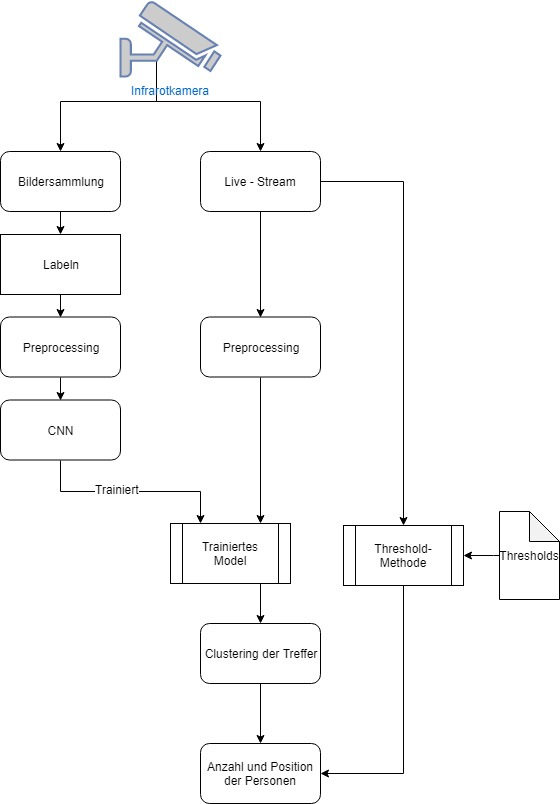
\includegraphics[width=.8\linewidth]{SystemOverview}
	\caption{Grobübersicht des Systems mit CNN- und Thresholdalgorithmus}
	\label{SystemOverview}
\end{figure}

\section{UDP-Schnittstelle}

Um die Bilder automatisiert erhalten zu können wurde eine Schnittstelle zu den Infrarotkameras implementiert. Es wurde das UDP-Protokoll verwendet, da die Kameras nur über dieses Protokoll angesprochen werden konnten.\\
 Die einzige ander Möglichkeit and Bilder zu gelangen wäre über die GUI Applikation des Herstellers Videos aufzunehmen. Dies sind bereits auf RGB convertiert, beihalten also nicht alle Information des ursprünglichen Bildes und die Applikation kann nicht automatisiert angesprochen werden. Folglich ist dies keine praktikable Variante um effizient Daten zu sammeln.\\
\\
Die Kameras können ausserdem nur mittels UDP-Broadcasts identifiziert und and einen Socket gebunden werden. Aus diesem Grund konnten die Kameras nicht im allgemeinen Schulnetzwerk installiert werden, sondern mussten in einem separaten Netzwerk betrieben werden. In diesem Netzwerk konnten sie über einen Computer angesteuert werden, der widerum mit dem HSLU-Netzwerk verbunden ist. Um die Entwicklung der Schnittstelle möglichst einfach zu gestalten wurde versucht einen Remoteinterpreter aufzusetzen. Dies ist eine funktion von Pycharm \parencite{pycharm} erlaubt es, auf einem Lokalen System zu entwickeln aber die Software direkt auf einem Remote System auszuführen und zu Debuggen.\\
Leider wird dies für Windows Remote Systeme nicht unterstützt. Deshalb wurde der Code jeweils manuell via sftp auf den Computer im Sitzungszimmer kopiert. Danach wurde mittel Windows Remotedesktopverbindung die Software ausgeführt und getestet. \\
\\
In einer ersten Variante wurde in dieser Schnittstelle mit Einzelbilder gearbeitet. Dies bietet den Vorteil, dass man die Bildrate einfah definieren und steuern kann. Leider war die Qualitiät dieser Bilder sehr schlecht. Durch eine Rücksprach mit dem Hersteller stellte sich heraus, das die Verwendung der Streaming Funktion der Kameras qualitativ besser Bilder liefert. Deshalb wurde die Schnittstelle auf die Verwendung von Streams abgeändert. Dabei war die Generator Funktionalität von Python sehr hilfreich. Die Eigenschaft von Generators, dass diese erst ausgeführt werden, wenn ein Objekt angefragt wird, konnte genutzt werden, um jederzeit das aktuellste Bild zu erhalten.

\section{Datensammlung}

Um die Trainingsdaten effizient zu sammeln wurde ein  Skript erstellt, welches von beiden Kameras gleichzeitig Bilder anfordert und Abspeichert. Dieses musste über mehrere Monate unterbruchlos laufen und wurde deshalb so Implementiert, dass es sich bei einem Fehler automatisch neu startet. Zusätzlich wurden parallel dazu auch Bilder der Referenzkamera aufgezeichnet, um das Labeling der Infrarotbilder zu vereinfachen und als Ground Truth zu verifizieren.\\
Alle aufgezeichneten Bilder wurden lokal auf einer Festplatte des Computers im Sitzungszimmer gespeichert. Um alle Bilder eindeutig zu identifizieren, wurden sie mit Art des Bildes, Infrarot oder Ground Truth, Zeitstempel und bei den Infrarotbildern mit Kamera 1 oder 2 versehen. Um das ganze übersichtlicher zu gestalten wurde das ganze in einem Ordnersystem abgelegt, das wie folgt aufgebaut ist.

\begin{itemize}
	\item ../ [Jahr] / [Monat] / [Tag] / [Bildtyp]\_[Uhrzeit]\_[Kamera].[Dateityp]
	\item Bsp.: ../2019/05/23/IR\_Image\_10\_33\_45\_2.npy
\end{itemize}


\section{Algorithmen}

Damit die beiden Algorithmen möglichst effizient und mit wenig Redundanz implementierte werden konnten, wurde die Software modular aufgebaut. Es wurde ein Package mit


\subsection{Testing}


\chapter{Evaluation und Validation}
\label{ch:Eval}

Um das System zu validieren und die Grenzen der Infrarotbildverarbeitung in diesem Gebiet zu ermitteln wurden einige Experimente durchgeführt. Diese Experimente zeigen, was das System kann und wo die Grenzen des Systems und auch der Infrarottechnik liegen.\\
\\
\section{Erklärungen}
\label{sec:explanation}
In diesem Kapitel werden Test statistisch ausgewertet und analysiert. Dazu werden hier die wichtigsten Begriffe und Konzepte erklärt.

\subsection{Farbcodierung}
Zur Auswertung der Experimente werden Bilder mit Markierungen verwendet. Diese sind wie folgt Farbcodiert.\\

\begin{itemize}
	\item \textbf{Grün:} Korrekt gefundene Person (True Positive)
	\item \textbf{Gelb:} Nicht gefundene Person (False Negative)
	\item \textbf{Rot:} Nichtiger Treffer (False Positive)
\end{itemize}
\vspace{1em}

\subsection{Begriffserklärung}
\noindent In dem Kapitel werden die folgenden Fachbegriffe verwendet:
\begin{itemize}
	\item $True\: Positive:$   Person wurde korrekt Identifiziert
	\item $True\: Negative:$   Hintergrund oder fremde Wärmequelle wurde \textbf{nicht} als Person identifiziert. Diese werden in diesem Kapitel nicht weiter verwendet, da diese der standard Fall ist und nicht spezifisch ausgewertet werden kann.
	\item $False\: Positive:$  Hintergrund oder fremde Wärmequelle wurde als Person identifiziert
	\item $False\: Negative:$  Person wurde nicht erkannt.
\end{itemize}
\vspace{1em}

\subsection{Statistische Metriken}
\noindent Zudem werden die folgenden Metriken verwendet, diese sind leicht angepasst, da die Klasse True Negative fehlt:

\begin{itemize}
	\item \textbf{Precision:} Korrekte Treffer / Alle Treffer\[\dfrac{True\: Positive}{True\: Positive + False\: Positive}\]
	\item \textbf{Recall/Accuracy:} Korrekte Treffer / Anzahl Personen\[\dfrac{True\: Positive}{True\: Positive + False\: Negative}\]
	\item \textbf{F1-Score:} \[\dfrac{2*Precision*Recall}{Precision + Recall}\]
\end{itemize}


\section{Vergleich mit Anforderungen}
\label{sec:VergleichAnforderungen}

Der erforderte Stand der Technik wurde in Kapitel \ref{ch:StandDerTechnik} präsentiert. Die gefundenen Algorithmen wurden in Kapitel \ref{ch:ideasAndConcepts} erklärt und evaluiert.\\
Das erste Hauptziel war es ein lauffähiges System zu entwickeln, welches die Position und Anzahl der Personen in einem Infrarotbild bestimmen kann. Dieses Ziel wurde mit einem Recall von 91.5\%  erreicht (siehe Tabelle \ref{tbl:stat}). Die beim betrachten der Werte in Tabelle \ref{tbl:results} und \ref{tbl:stat} ist zu beachten, dass dabei auch die Grenzen des Systems getestet wurden. So zum Beispiel in Kapitel \ref{sec:cloths} wo der Einfluss isolierender Kleidung analysiert wird.\\
Das zweite Hauptziel ist es Schwierigkeiten bei der Lösung der Aufgabe zu erläutern und Lösungsmöglichkeiten dazu vorzuschlagen. Dies wird in diesem Kapitel und im Kapitel \ref{ch:Ausblick} erfüllt.

% Tabelle mit ergebnissen
{
	\renewcommand{\arraystretch}{1.3}
	
	\begin{table}[H]
		\scriptsize
		\centering
		\begin{tabularx}{.5\textwidth}{Xrr}\\
			\hline
			\multicolumn{3}{c}{\textbf{Ergebnisse der Algorithmen}}\\
			\hline
			\textbf{Kategorien} & \textbf{CNN} & \textbf{Threshold}\\
			\hline
			\textit{Anzahl verwendeter Aufnahmen} & 323 & 323\\
			\hline 
			\textit{Gesamtanzahl Personen in Bilder} & 718 & 718\\
			\hline
			\textit{True Positive} & 657 & 650\\
			\hline
			\textit{False Positive} & 120 & 142\\
			\hline
			\textit{False Negative} & 61 & 68\\
		\end{tabularx}
		\caption{Zusammenfassung der Ergebnisse beider Algorithmen}
		\label{tbl:results}
	\end{table}
	\begin{table}[H]
		\scriptsize
		\centering
		\begin{tabularx}{.5\textwidth}{Xrr}
			\hline
			\multicolumn{3}{c}{\textbf{Statistische Auswertung}}\\
			\hline
			\textbf{Kategorien} & \textbf{CNN} & \textbf{Threshold}\\
			\hline
			\textit{Recall} & 91.5\% & 90.5\%\\
			\hline  
			\textit{Precision} & 84.5\% & 82.1\%\\
			\hline
			\textit{F1-Score} & 87.9\% & 86.1\%\\
			\hline
		\end{tabularx}
		\caption{Statistische Auswertung der Performance beider Algorithmen}
		\label{tbl:stat}
	\end{table}
}

\section{Fremde Wärmequellen}
\label{sec:FremdeWärmequellen}

In diesem Versuch wurde der Einfluss von fremden Wärmequellen, wie zum Beispiel Laptops, Natels, Kaffees oder Radiatoren, evaluiert. Dabei wurde der Effekt von Störquellen mit und ohne Personen im Raum analysiert.

\subsection{Versuchsaufbau}

Um die Performance der Algorithmen spezifisch in Bezug auf fremde Wärmequellen zu testen, wurden verschiedene Testsituationen erzeugt. Zuerst wurden fünf Laptops, von 13" bis 17",auf den Sitzungstisch gestellt, um zu sehen, ob Laptops ohne Personen Treffer generieren. Die Geräte wurden auf den gesamten Kamerawinkel verteilt, vom Zentrum des Bildes bis an den Rand. Da die Algorithmen nicht durch die Anzahl Wärmequellen, sondern nur durch die Distanz zwischen den Wärmequellen beeinflusst werden, konnte der ganze Kamerawinkel in einem einzigen Versuch getestet werden.\\
Die Temperatur der Laptops wurde von der Infrarotkamera als ca. 25\degree C erfasst, somit etwas unter der Abstrahlungswärme einer Person. Die Hauttemperatur einer Person wird von den Infrarotkameras zwischen 27\degree C und 33\degree C gemessen, je nach Kleidung und Behaarung.\\
Danach nahmen fünf Personen bei den Laptops platz,  ohne dass die Laptops verschoben wurde. Um zu testen, ob False Positives generiert werden, wenn jemand den Laptop bedient, die Arme zum Laptop reichen.\\
Um auch Wärmere Laptops überprüfen zu können wurde Bilder während einer Besprechung aufgezeichnet. Dabei war ein Laptop, dessen Temperatur im Bereich der Hauttemperatur einer Person liegt, in der Mitte des Tischs, ein anderer nahe bei einer Person. Die Szene ist in Abbildung \ref{fig:exampleDeviceTest2} zu sehen.
\\
\begin{figure}[htb]
	\centering
	\begin{subfigure}{.45\linewidth}
		\centering
		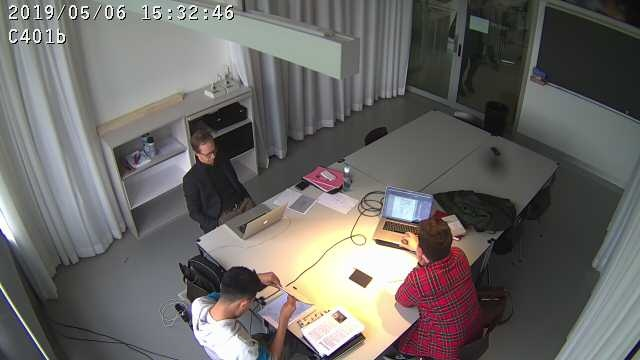
\includegraphics[keepaspectratio, height=4cm]{groundDeviceTest2}
	\end{subfigure}
	\begin{subfigure}{.45\linewidth}
		\centering
		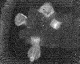
\includegraphics[keepaspectratio, height=4cm]{exampleDeviceTest2}
	\end{subfigure}
	\caption{Ansicht des Sitzungszimmers während der Aufnahme des zusätzlichen Laptop- und Personen-Testsets}
	\label{fig:exampleDeviceTest2}
\end{figure}
Schon bei der Erstellung der Modelle wurde ersichtlich, dass das Herausfiltern von Wärmequellen mit sehr kleiner Fläche für beide Algorithmen kein Problem darstellt. Aus diesem Grund wurden die Versuche mit kleineren Wärmequellen nur in kleinem Rahmen durchgeführt. Es wurde Test mit einem Mobiltelefon durchgeführt, in dem ein Natel an verschiedenen Postionen auf den Tisch gelegt wurde. Da Mobiltelefone meist in der Hosentasche getragen werden, weisen diese Temperaturen bis zu 34\degree C auf.\\
\\

\subsection{Resultate}

{
	\renewcommand{\arraystretch}{1.3}
	\begin{table}[H]
		\centering
		\scriptsize
		\begin{tabularx}{.9\textwidth}{Xrrrr}
			\hline
			\multicolumn{5}{c}{\textbf{\gls{CNN} Ergebnisse Fremde Wärmequellen}}\\
			\hline
			\textbf{Metriken} & \textbf{Nur Laptops} & \textbf{Laptops mit Personen} & \textbf{Mobiltelefon} & \textbf{Radiator}\\
			\hline 
			\textbf{Gesamtanzahl Personen in Bilder} & 0 & 39 & 0 & 20\\
			\hline
			\textbf{Korrekt identifizierter Personen} & 0 & 39 & 0 & 20\\
			\hline
			\textbf{Falsche Treffer} & 1 & 0 & 0 & 27\\
			\hline
			\textbf{Nicht erkannte Personen} & 0 & 0 & 0 & 0\\
			\hline
			\textbf{Recall} & -- & 100\% & -- & 100\%\\
			\hline  
			\textbf{Precision} & -- & 100\% & -- & 42.6\%\\
			\hline
			\textbf{F1-Score} & -- & 100\% & -- & 59.7\%\\
			\hline
		\end{tabularx}
		\caption{Ergebnisse des \gls{CNN}, der Experimente mit fremden Wärmequellen}
		\label{tbl:heatSourcesCNN}
	\end{table}
	\begin{table}[H]
		\centering
		\scriptsize
		\begin{tabularx}{.9\textwidth}{Xrrrr}
			\hline
			\multicolumn{5}{c}{\textbf{Threshold-Methode Ergebnisse Fremde Wärmequellen}}\\
			\hline
			\textbf{Metriken} & \textbf{Nur Laptops} & \textbf{Laptops mit Personen} & \textbf{Mobiltelefon} & \textbf{Radiator}\\
			\hline 
			\textbf{Gesamtanzahl Personen in Bilder} & 0 & 39 & 0 & 20\\
			\hline
			\textbf{Korrekt identifizierter Personen} & 0 & 33 & 0 & 20\\
			\hline
			\textbf{Falsche Treffer} & 1 & 014 & 16 & 87\\
			\hline
			\textbf{Nicht erkannte Personen} & 0 & 0 & 0 & 0\\
			\hline
			\textbf{Recall} & -- & 84.6\% & -- & 100\%\\
			\hline  
			\textbf{Precision} & -- & 70.2\% & -- & 18.7\%\\
			\hline
			\textbf{F1-Score} & -- & 76.7\% & -- & 31.5\%\\
			\hline
		\end{tabularx}
		\caption{Ergebnisse, der Threshold-Methode, der Experimente mit fremden Wärmequellen}
		\label{tbl:heatSourcesThresh}
	\end{table}
}

\subsection{Evaluation}

Die Threshold-Methode kann, wie erwartet, nicht gut mit anderen Wärmequellen umgehen. Dies, weil die Threshold-Methode nur durch Temperatur und Mindestgrösse eines Objekts entscheiden kann, ob es sich um eine Person handelt oder nicht. Deshalb hatte dieser auf den Testbildern mit Personen und Laptops, nur eine Precision Score von 70\% erreicht und bei dem Versuch mit Radiator auf hoher Stufe sogar nur eine von 18.7\% (Siehe Abbildungen  \ref{fig:ThreshPersonLaptop} und \ref{fig:thresholdRadiator}).\\
\\
Das \gls{CNN} kann gut mit anderen Wärmequellen umgehen, solange diese in ähnlicher Form antrainiert wurden (siehe Abbildung \ref{fig:cnnPersonLaptop}. Ist dies jedoch nicht der Fall und die Wärmequelle ist dem \gls{CNN} nicht in ähnlicher Form bekannt tendiert es dazu diese, wenn sie etwas grösser sind, als Personen zu identifizieren, was in Abbildung \ref{fig:cnnRadiator} zu sehen ist. Eine Lösung zu diesem Problem wird in Kapitel \ref{ch:Ausblick} diskutiert. 

\vspace{.5em}
\begin{figure}[htb]
	\centering
	\begin{subfigure}{.45\linewidth}
		\centering
		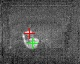
\includegraphics[keepaspectratio,height=4cm]{ThreshPersonLaptop}
		\caption{Ergebnis der Threshold-Methode des Experiments mit Laptop und Person}
		\label{fig:ThreshPersonLaptop}
	\end{subfigure}\hfill%
	\begin{subfigure}{.45\linewidth}
		\centering
		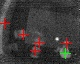
\includegraphics[keepaspectratio,height=4cm]{threshRadiator}
		\caption{Threshold-Methode Ergebnis des Radiator Experiments}
		\label{fig:thresholdRadiator}
	\end{subfigure}\hfill%
	\begin{subfigure}{.45\linewidth}
		\centering
		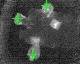
\includegraphics[keepaspectratio,height=4cm]{cnnPersonLaptop}
		\caption{CNN Ergebnis des Experiments mit Laptops und Personen}
		\label{fig:cnnPersonLaptop}
	\end{subfigure}\hfill%
	\begin{subfigure}{.45\linewidth}
		\centering
		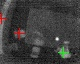
\includegraphics[keepaspectratio, height=4cm]{cnnRadiator}
		\caption{CNN Ergebnis des Radiator Experiments}
		\label{fig:cnnRadiator}
	\end{subfigure}\hfill%
	\begin{subfigure}{.55\linewidth}
		\centering
		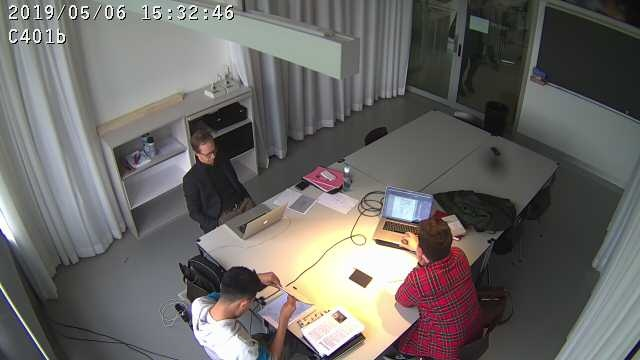
\includegraphics[keepaspectratio,height=3cm]{groundDeviceTest2}
		\caption{Ground-Truth des Experiments mit Laptop und Person}
		\label{fig:groundPersonLaptop}
	\end{subfigure}
	\caption{Experimente mit fremden Wärmequellen}
	\label{fig:HeatSources}
\end{figure}
\vspace{.5em}



\section{Distanz}
\label{sec:distanz}

Die Distanz zwischen zwei Personen ist ein wichtiger Faktor, der auf beide Algorithmen Einfluss hat. Da bei dem \gls{CNN} mit einer Sliding-Window Methode und Clustern der Treffer gearbeitet wird, kann das System, bei Personen, welche zu wenig Abstand zueinander haben, die Treffer nicht mehr auseinanderhalten. Bei der Threshold-Methode wird die Silhouette der Personen leicht vergrössert, wodurch mehrere Personen bei geringem Abstand als einzelner Treffer gewertet werden können.

\subsection{Versuchsaufbau}

Es wurden vier Personen in zwei Paaren so platziert, dass sich das eine Paar in einem idealen Winkel zur Infrarotkamera aufhält und das andere Paar in einem möglichst schwierigen Winkel. Dies ist in Abbildung \ref{fig:cnnDistance10} gut zu sehen. Zwei Personen sind deutlich voneinander getrennt, die anderen zwei überlappen sich aufgrund des Kamerawinkels. Diese Versuchsanordnung wurde gewählt, um in einem Test beide Extreme überprüfen zu können. 
Beim Test wurde schrittweise der Abstand zwischen den Testpersonen erhöht, um festzustellen, ab welcher Distanz die Algorithmen erfolgreich die Personen erkennen. Der Abstand wird in 10cm Schritten erhöht, weil 10cm auf Tischhöhe ca. einem Pixel auf dem Bild entspricht.

\subsection{Resultate}

{
	\renewcommand{\arraystretch}{1.3}
	\begin{table}[H]
		\centering
		\scriptsize
		\begin{tabularx}{.9\textwidth}{Xrrrrrr}
			\hline
			\multicolumn{7}{c}{\textbf{\gls{CNN} Ergebnisse Distanz Experiment}}\\
			\hline
			\textbf{Metriken} & \textbf{10cm} & \textbf{20cm} & \textbf{30cm} & \textbf{40cm} & \textbf{50cm} & \textbf{60cm}\\
			\hline 
			\textbf{Gesamtanzahl Personen in Bilder} & 29 & 18 & 54 & 18 & 51 & 28\\
			\hline
			\textbf{Korrekt identifizierter Personen} & 29 & 18 & 54 & 18 & 51 & 28\\
			\hline
			\textbf{Falsche Treffer} & 0 & 0 & 0 & 0 & 0 & 0\\
			\hline
			\textbf{Nicht erkannte Personen} & 0 & 0 & 0 & 0 & 0 & 0\\
			\hline
			\textbf{Recall} & 100\% & 100\% & 100\% & 100\% & 100\% & 100\%\\
			\hline  
			\textbf{Precision} & 100\% & 100\% & 100\% & 100\% & 100\% & 100\%\\
			\hline
			\textbf{F1-Score} & 100\% & 100\% & 100\% & 100\% & 100\% & 100\%\\
			\hline
		\end{tabularx}
		\caption{Ergebnisse des \gls{CNN}, der Distanz Experimente}
		\label{tbl:distanceCNN}
	\end{table}
	\begin{table}[H]
		\centering
		\scriptsize
		\begin{tabularx}{.9\textwidth}{Xrrrrrr}
			\hline
			\multicolumn{7}{c}{\textbf{Threshold-Methode Ergebnisse Distanz Experiment}}\\
			\hline
			\textbf{Metriken} & \textbf{10cm} & \textbf{20cm} & \textbf{30cm} & \textbf{40cm} & \textbf{50cm} & \textbf{60cm}\\
			\hline 
			\textbf{Gesamtanzahl Personen in Bilder} & 29 & 18 & 54 & 18 & 51 & 28\\
			\hline
			\textbf{Korrekt identifizierter Personen} & 22 & 15 & 54 & 18 & 51 & 28\\
			\hline
			\textbf{Falsche Treffer} & 4 & 1 & 3 & 1 & 3 & 1\\
			\hline
			\textbf{Nicht erkannte Personen} & 7 & 3 & 0 & 0 & 0 & 0\\
			\hline
			\textbf{Recall} & 75.9\% & 83.3\% & 100\% & 100\% & 100\% & 100\%\\
			\hline  
			\textbf{Precision} & 84.6\% & 93.8\% & 94.7\% & 94.7\% & 94.4\% & 100\%\\
			\hline
			\textbf{F1-Score} & 80.0\% & 88.2\% & 97.2\% & 97.2\% & 97.1\% & 100\%\\
			\hline
		\end{tabularx}
		\caption{Ergebnisse, der Threshold-Methode, der Distanz Experimente}
		\label{tbl:distanceThresh}
	\end{table}
}

\subsection{Evaluation}


Das \gls{CNN} Kann bereits ab einem Abstand von 10cm zuverlässig Personen auseinanderhalten.\\
Die Threshold-Methode kann Personen bereits ab einem Abstand von 10cm auseinanderhalten, sofern die Personen so ausgerichtet sind, dass die optische Verzerrung keinen Einfluss auf den Zwischenraum hat. Wie in der Abbildung \ref{fig:thresholdDistance10} in der linken Bildhälfte zu sehen ist, können die Personen, die auf die Kamera ausgerichtet sind, unterschieden werden. Sind die Person jedoch so platziert, wie auf der rechten Bildhälfte zu sehen ist, sind diese von der Kamera aus gesehen, hintereinander. Bei dieser geringen Distanz kann der Algorithmus deshalb nicht mehr bestimmen, ob es sich um eine oder mehrere Personen handelt.\\
Befinden sich die Personen in der schlechtestmöglichen Position, benötigt die Threshold-Methode einen Mindestabstand von 30cm, um die Personen fehlerfrei unterscheiden zu können (siehe Abbildung \ref{fig:thresholdDistance30}).

\begin{figure}[H]
	\begin{subfigure}{.45\linewidth}
		\centering
		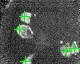
\includegraphics[keepaspectratio,height=4cm]{CNNDistance10}
		\caption{\gls{CNN} Ergebnis des Distanztest mit 10cm Abstand}
		\label{fig:cnnDistance10}
	\end{subfigure}\hfill%
	\begin{subfigure}{.45\linewidth}
		\centering
		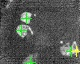
\includegraphics[keepaspectratio,height=4cm]{threshDistance10}
		\caption{Threshold Ergebnis des Distanztest mit 10cm Abstand}
		\label{fig:thresholdDistance10}
	\end{subfigure}\hfill
	\begin{subfigure}{\linewidth}
		\centering
		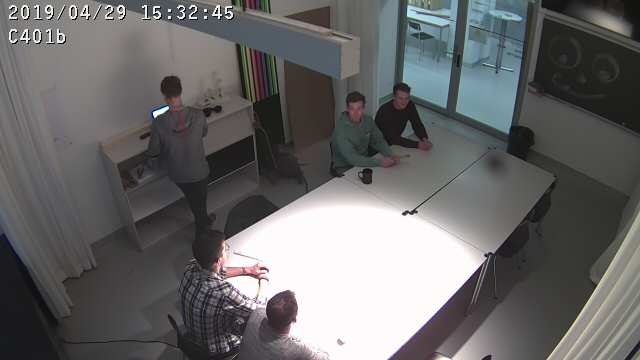
\includegraphics[keepaspectratio,height=3cm]{GroundDistance10}
		\caption{Ground-Truth Distanzexperiment mit 10cm Abstand}
		\label{fig:groundDistance10}
	\end{subfigure}
	\caption{Distanzexperiment 10cm}
	\label{fig:Distance10}
\end{figure}

\begin{figure}[H]
	\begin{subfigure}{.45\linewidth}
		\centering
		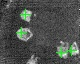
\includegraphics[keepaspectratio,height=4cm]{CNNDistance30}
		\caption{\gls{CNN} Ergebnis des Distanztest mit 30cm Abstand}
		\label{fig:cnnDistance30}
	\end{subfigure}\hfill%
	\begin{subfigure}{.45\linewidth}
		\centering
		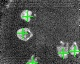
\includegraphics[keepaspectratio,height=4cm]{threshDistance30}
		\caption{Threshold Ergebnis des Distanztest mit 30cm Abstand}
		\label{fig:thresholdDistance30}
	\end{subfigure}\hfill%
	\begin{subfigure}{\linewidth}
		\centering
		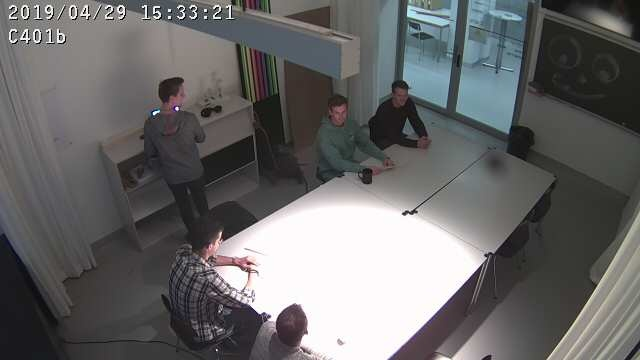
\includegraphics[keepaspectratio,height=3cm]{GroundDistance30}
		\caption{Ground-Truth}
		\label{fig:groundDistance30}
	\end{subfigure}
	\caption{Distanzexperiment 30cm}
	\label{fig:Distance30}
\end{figure}

\section{Grösse Des Objekts auf dem Bild}
\label{sec:objectSize}
Eine Spezialität des Sitzungszimmers, das zur Verfügung gestellt wurde, ist, dass die Höhe der Decke verändert werden kann. Da die Infrarotkameras an der Decke montiert sind, wurde dies als Möglichkeit genutzt um zu testen wie die Algorithmen auf grössen der Objekte im Bild reagieren. 

\subsection{Versuchsaufbau}

Die verstellbare Decke des Sitzungszimmers wurde auf die vom Mobiliar zugelassene Minimalhöhe, ca. 255cm, heruntergefahren. Danach wurden Infrarotbilder von Testpersonen an verschiedenen Positionen aufgenommen (siehe Abbildung \ref{fig:ground255cm}). Anschliessend wurde die Decke maximal hochgefahren, etwa 400cm, und noch einmal Bilder aufgezeichnet.

\begin{figure}[H]
	\centering
	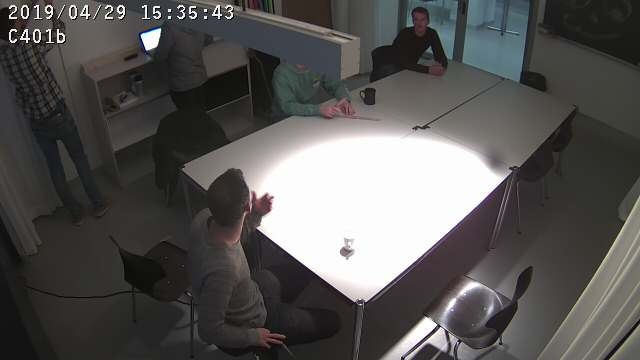
\includegraphics[height=4cm]{ground255cm}
	\caption{Sitzungszimmer mit Decke auf 255cm}
	\label{fig:ground255cm}
\end{figure}

\subsection{Resultate}

{
	\renewcommand{\arraystretch}{1.3}
	\begin{table}[H]
		\scriptsize
		\centering
		\begin{tabularx}{.6\textwidth}{Xrr}
			\hline
			\multicolumn{3}{c}{\textbf{CNN Ergebnisse des Objektgrössenexperiments}}\\
			\hline
			\textbf{Metriken} & \textbf{255cm} & \textbf{400cm}\\
			\hline
			\textbf{Gesamtanzahl Personen in Bilder} & 78 & 44 \\
			\hline
			\textbf{Korrekt identifizierter Personen} & 77 & 42\\
			\hline
			\textbf{Falsche Treffer} & 7 & 1\\
			\hline
			\textbf{Nicht erkannte Personen} & 1 & 2\\
			\hline
			\textbf{Recall} & 98.7\% & 95.5\%\\
			\hline  
			\textbf{Precision} & 91.7\% & 97.7\%\\
			\hline
			\textbf{F1-Score} & 95.1\% & 96.6\%\\
			\hline
		\end{tabularx}
		\caption{CNN, Ergebnisse des Distanztests}
		\label{tbl:objectSizeCNN}
	\end{table}
	\begin{table}[H]
		\scriptsize
		\centering
		\begin{tabularx}{.6\textwidth}{Xrr}
			\hline
			\multicolumn{3}{c}{\textbf{Threshold-Methode Ergebnisse des Objektgrössenexperiments}}\\
			\hline
			\textbf{Metriken} & \textbf{255cm} & \textbf{400cm}\\
			\hline
			\textbf{Gesamtanzahl Personen in Bilder} & 78 & 44 \\
			\hline
			\textbf{Korrekt identifizierter Personen} & 77 & 44\\
			\hline
			\textbf{Falsche Treffer} & 8 & 1\\
			\hline
			\textbf{Nicht erkannte Personen} & 1 & 0\\
			\hline
			\textbf{Recall} & 98.7\% & 100\%\\
			\hline  
			\textbf{Precision} & 90.6\% & 97.8\%\\
			\hline
			\textbf{F1-Score} & 94.5\% & 98.9\%\\
			\hline
		\end{tabularx}
		\caption{Threshold-Methode, Ergebnisse des Distanztests}
		\label{tbl:objectSizeThresh}
	\end{table}
}

\subsection{Evaluation}
Beide Algorithmen können die Personen in beiden Situationen noch immer in über 95\% der Fälle identifizieren. Werden die Objekte jedoch zu gross kann es bei beiden dazu führen, dass Personen doppelt gezählt werden. Da eine solch kleine Distanz aber nur schon durch das sehr kleine Sichtfeld für einen solchen Anwendungsfall nicht praktikabel ist, ist dies kein Problem, das weiter verfolgt werden müsste.\\
Werden die Objekte kleiner stellt dies für beide Algorithmen kein messbares Problem dar, solange die Charakteristiken noch klar erkennbar sind und die Personen eine Fläche von mindestens 10x10 Pixel einnehmen. Ein Test um die Grenze in diesem Bereich zu testen konnte in den zur Verfügung stehenden Räumlichkeiten leider nicht durchgeführt werden.\\
Möchte man jedoch die reale Position der Personen aus dem Bild berechnen, müsste die Deckenhöhe zusätzlich berechnet oder gemessen werden.

\begin{figure}[H]
	\begin{subfigure}{.45\linewidth}
		\centering
		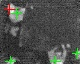
\includegraphics[keepaspectratio, height=4cm]{CNN255}
		\caption{Ergebnis des CNN mit Deckenhöhe 255cm}
		\label{fig:cnn255}
	\end{subfigure}\hfill%
	\begin{subfigure}{.45\linewidth}
		\centering
		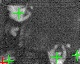
\includegraphics[keepaspectratio, height=4cm]{thresh255}
		\caption{Ergebnis der Threshold-Methode mit Deckenhöhe 255cm}
		\label{fig:thresh255}
	\end{subfigure}\hfill%
	\begin{subfigure}{.45\linewidth}
		\centering
		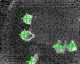
\includegraphics[keepaspectratio, height=4cm]{CNN400}
		\caption{Ergebnis des CNN mit Deckenhöhe 400cm}
		\label{fig:cnn400}
	\end{subfigure}\hfill%
	\begin{subfigure}{.45\linewidth}
		\centering
		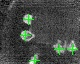
\includegraphics[keepaspectratio, height=4cm]{thresh400}
		\caption{Ergebnis der Threshold-Methode mit Deckenhöhe 400cm}
		\label{fig:thresh400}
	\end{subfigure}\hfill%
	\begin{subfigure}{.45\linewidth}
		\centering
		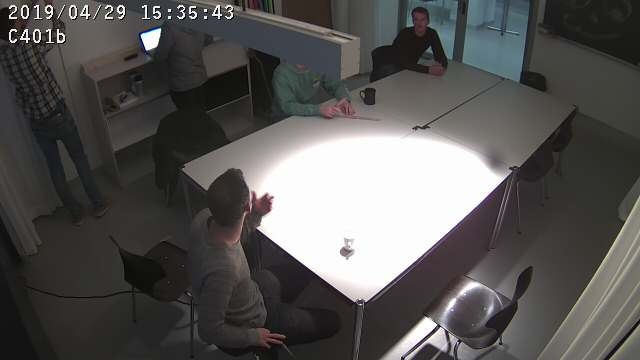
\includegraphics[keepaspectratio, height=4cm]{ground255cm}
		\caption{Ground Truth Deckenhöhe 255cm}
		\label{fig:ground255}
	\end{subfigure}\hfill%
	\begin{subfigure}{.45\linewidth}
		\centering
		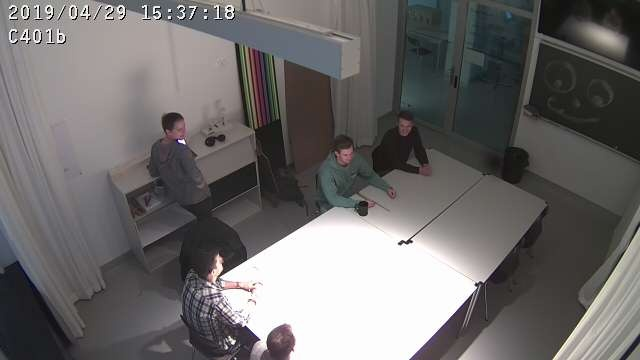
\includegraphics[keepaspectratio, height=4cm]{ground400cm}
		\caption{Ground Truth Deckenhöhe 400cm}
		\label{fig:ground400}
	\end{subfigure}
\end{figure}


\section{Kleider}
\label{sec:cloths}

Infrarotbilder zeigen die Wärmeabstrahlung der verschiedenen Objekte im Bild. Wird eine Wärmequelle isoliert, verschwindet sie auf dem Infrarotbild. Genau das passiert, wenn stark isolierende Kleider getragen werden. Da in dieser Arbeit die Vogelperspektive analysiert wird, haben vor allem Kopfbedeckungen, Schals und Jacken einen grossen Einfluss. 

\subsection{Versuchsaufbau}

Eine Testperson hielt sich an den in den Abbildungen \ref{fig:clothPositions} zu sehenden Positionen im Raum auf und trug verschiedene Kleidungsstücke. Dabei wurden eine Mütze, ein Schal und eine Jacke einzeln und alle kombiniert von der Testperson getragen.

\begin{figure}[H]
	\centering
	\begin{subfigure}{.45\linewidth}
		\centering
		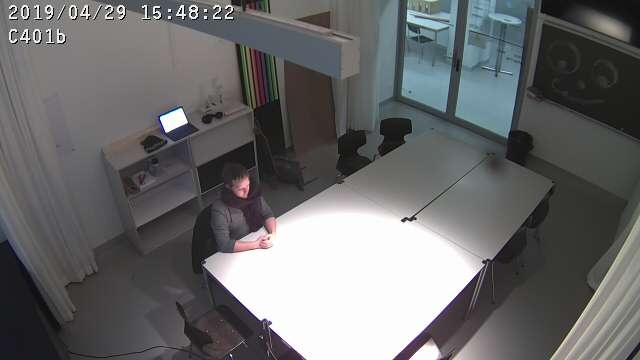
\includegraphics[keepaspectratio, height=3cm]{clothPos1}
		\caption{Position 1}
	\end{subfigure}
	\begin{subfigure}{.45\linewidth}
		\centering
		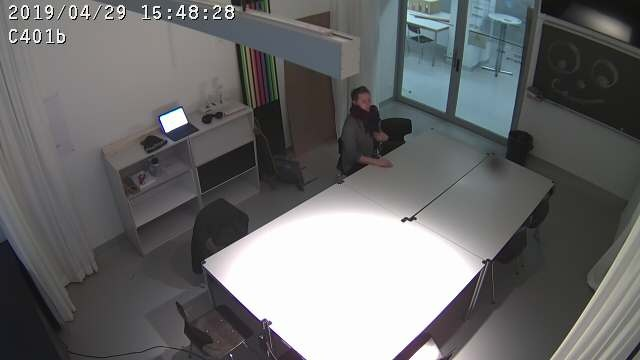
\includegraphics[keepaspectratio, height=3cm]{clothPos2}
		\caption{Position 2}
	\end{subfigure}
	\begin{subfigure}{.45\linewidth}
		\centering
		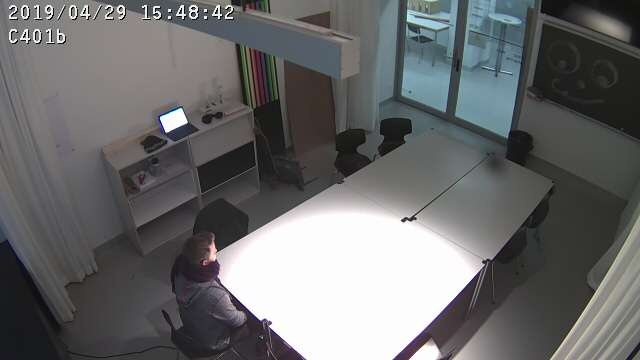
\includegraphics[keepaspectratio, height=3cm]{clothPos3}
		\caption{Position 3}
	\end{subfigure}
	\caption{Positionen der Testperson im Kleidungs Experiment}
	\label{fig:clothPositions}
\end{figure}

\subsection{Resultate}

{
	\renewcommand{\arraystretch}{1.3}
	\begin{table}[H]
		\centering
		\scriptsize
		\begin{tabularx}{.9\textwidth}{Xrrrr}
			\hline
			\multicolumn{5}{c}{\textbf{CNN Ergebnisse Kleider Experiment}}\\
			\hline
			\textbf{Metriken} & \textbf{Kappe} & \textbf{Jacke} & \textbf{Schaal} & \textbf{Alle drei Kleidungsstücke}\\
			\hline 
			\textbf{Gesamtanzahl Personen in Bilder} & 19 & 18 & 21 & 3\\
			\hline
			\textbf{Korrekt identifizierter Personen} & 23 & 0 & 15 & 0\\
			\hline
			\textbf{Falsche Treffer} & 0 & 0 & 0 & 0\\
			\hline
			\textbf{Nicht erkannte Personen} & 4 & 18 & 6 & 3\\
			\hline
			\textbf{Recall} & 82.6\% & -- & 71.4\% & -- \\
			\hline  
			\textbf{Precision} & 100\% & -- & 100\% & -- \\
			\hline
			\textbf{F1-Score} & 90.5\% & -- & 83.3\% & -- \\
			\hline
		\end{tabularx}
		\caption{Ergebnisse des CNN, des Kleider Experiments}
		\label{tbl:clothCNN}
	\end{table}
	\begin{table}[H]
		\centering
		\scriptsize
		\begin{tabularx}{.9\textwidth}{Xrrrr}
			\hline
			\multicolumn{5}{c}{\textbf{CNN Ergebnisse Kleider Experiment}}\\
			\hline
			\textbf{Metriken} & \textbf{Kappe} & \textbf{Jacke} & \textbf{Schaal} & \textbf{Alle drei Kleidungsstücke}\\
			\hline 
			\textbf{Gesamtanzahl Personen in Bilder} & 23 & 18 & 21 & 3\\
			\hline
			\textbf{Korrekt identifizierter Personen} & 23 & 5 & 16 & 0\\
			\hline
			\textbf{Falsche Treffer} & 12 & 0 & 1 & 3\\
			\hline
			\textbf{Nicht erkannte Personen} & 4 & 13 & 5 & 0\\
			\hline
			\textbf{Recall} & 100\% & 27.8\% & 76.2\% & -- \\
			\hline  
			\textbf{Precision} & 65.7\% & 100\% & 94.1\% & -- \\
			\hline
			\textbf{F1-Score} & 79.3\% & 43.5\% & 84.2\% & -- \\
			\hline
		\end{tabularx}
		\caption{Ergebnisse der Threshold-Methode, des Kleider Experiments}
		\label{tbl:clothThresh}
	\end{table}
}



\subsection{Evaluation}
Kleider beeinflussen die Performance der Algorithmen massiv. Trägt eine Person z.B. eine Mütze, wird sie vom \gls{CNN} noch zu 83\% erkannt. Bei der Threshold-Methode sind es zwar 100\%,führt aber dazu, dass eine Person zwei Treffer erzeugt (siehe Abbildung \ref{fig:thresholdClothHat}).\\
\\
Wenn ein Schal getragen wird, sinkt der Recall auf 71\% beim \gls{CNN} und 76\% bei der Threshold-methode. Betrachtet man Abbildung \ref{fig:scarfIR} sieht man deutlich, wie der Schal einen Teil der Wärme der Person verdeckt.\\
\\
Das Tragen einer Jacke macht es für die Algorithmen beinahe unmöglich die Personen zu erkennen. Die Person wird nur noch in wenigen Fällen erkannt. Da die Fläche der Abwärme einer Person so nur noch wenige Pixel beträgt, wird es schwierig diese von fremden Wärmequellen zu unterscheiden.\\

\begin{figure}[H]
	\centering
	\begin{subfigure}{.45\linewidth}
		\centering
		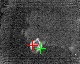
\includegraphics[keepaspectratio, height=4cm]{thresholdClothHat}
		\caption{Resultat der Threshold-Methode des Experiments mit Kopfbedeckung}
		\label{fig:thresholdClothHat}
	\end{subfigure}\hfill%
	\begin{subfigure}{.45\linewidth}
		\centering
		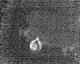
\includegraphics[keepaspectratio, height=4cm]{scarfIR}
		\caption{Infrarotbild einer Person die einen Schal trägt}
		\label{fig:scarfIR}
	\end{subfigure}\hfill%
	\caption{Infrarotbilder aus dem Kleider Experiment}
\end{figure}

\noindent
Die Tests mit allen Kleidungsstücken zeigen schon bei der manuellen, visuellen Analyse der Abbildung \ref{fig:rawClothAll}, dass wenn Jacke, Mütze und Schal zusammen getragen werden, dass die Person nicht mehr erkennbar ist.

\begin{figure}[H]
	\begin{subfigure}{.45\linewidth}
		\centering
		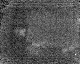
\includegraphics[keepaspectratio, height=4cm]{rawClothAll}
		\caption{Infrarotbild des Experiments mit Jacke, Mütze und Schal}
		\label{fig:rawClothAll}
	\end{subfigure}\hfill%
	\begin{subfigure}{.45\linewidth}
		\centering
		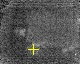
\includegraphics[keepaspectratio, height=4cm]{clothAll}
		\caption{Position der Person}
		\label{fig:AlgorithmsClothAll}
	\end{subfigure}\hfill%
	\begin{subfigure}{\linewidth}
		\centering
		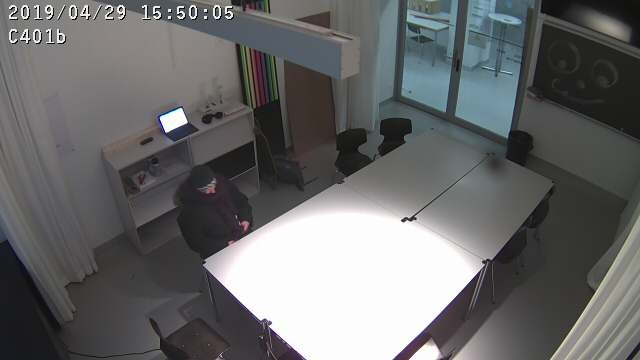
\includegraphics[keepaspectratio, width=.5\linewidth]{GroundClothAll}
		\caption{Ground-Truth des Experiments mit allen Kleidern}
		\label{fig:groundTruthClothAll}
	\end{subfigure}
	\caption{Experiment mit Jacke Mütze und Schal}
	\label{fig:AllCloth}
\end{figure}



\chapter{Fazit und Ausblick}
\label{ch:Ausblick}

Zum Abschluss wird in diesem Kapitel über die Arbeit reflektiert und diskutiert wie ein solches Projekt weitergeführt werden könnte und welche Verbesserungs- oder Erweiterungsmöglichkeiten es gibt.

\section{Technisches Fazit}

Technisch wurden die Anforderungen erfüllt. Leider ist es jedoch nicht gelungen ein System zu entwickeln , welches zuverlässig Personen von anderen Wärmequellen unterscheiden kann. Das \gls{CNN} ist darin zwar besser als die Threshold Methode, leider kann es aber auch nicht in allen Fällen korrekt entscheiden. Dieses Problem könnte durch Training mit mehr Daten oder mehr spezifischen Klassen minimiert werden. %TODO write more

\section{Projekt Fazit}

Das Projekt war rückblickend gesehen erfolgreich. Auch wenn das entwickelte System nicht mit hundertprozentiger Genauigkeit arbeitet, konnte gezeigt werden, wo die Herausforderungen liegen und was getan werden kann, um diese zu meistern. Es wurde gezeigt, dass das Erkennen von Personen relativ einfach ist, das Unterscheiden von Personen von anderen Wärmequellen hingegen eine Herausforderung darstellt. Da bei so kleiner Auflösung sehr wenig Information zur Verfügung steht und Personen viele verschiedene Haltungen einnehmen können (siehe Abbildung \ref{fig:postureExample}), ist es schwierig ein perfektes Modell dazu zu erstellen.

\begin{figure}[H]
	\centering
	\begin{subfigure}{.4\linewidth}
		\centering
		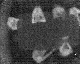
\includegraphics[keepaspectratio, height=4cm]{postureExample1}
	\end{subfigure}
	\begin{subfigure}{.4\linewidth}
		\centering
		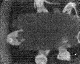
\includegraphics[keepaspectratio, height=4cm]{postureExample2}
	\end{subfigure}	
	\caption{Beispielbilder Haltung}
	\label{fig:postureExample}
\end{figure}

\subsection{Persönliches Fazit}

Ich sehe das Projekt auch persönlich als einen Erfolg an. Ich werde bestimmt viele Dinge mitnehmen die ich während des Projekts gelernt habe. Natürlich verlief auch in diesem Projekt nicht immer alles nach Plan und ich musste Zeit in die Lösung von Problemen investieren, die nicht direkt das System betrafen. Doch alles in allem konnte ich ein funktionierendes System entwickeln, welches mit einer 92\% Sicherheit und 93\% Präzision Personen erkennt und deren Position bestimmen kann.

\section{Ausblick}
Um dieses Projekt erfolgreich weiterzuführen und auszubauen, könnte man das \gls{CNN} durch einen grösseren Trainingsdatensatz von mindestens 1000 Bildern jeder Klasse verbessern. Auch wäre es angebracht zu evaluieren, ob mehr und spezifischere Klassen sinnvoll wären. Die momentane Fremde-Wärmequellen-Klasse beinhaltet sehr verschiedene Objekte, wie Laptops, Kaffees oder die erwärmte Fensterbank. Würde man dies feiner granulieren, könnte das \gls{CNN} sie besser erkennen.\\
Die Threshold-Methode hingegen bietet kaum Optimierungspotenzial. Man könnte einzig noch umgebungsspezifische Anpassungen vornehmen, zum Beispiel könnte die Fensterbank oder der Bereich des Sitzungstisches ausgeschlossen werden. Diese Methode ist jedoch sehr anfällig auf Änderungen im Raum, wird beispielsweise der Tisch verschoben, so funktioniert der Algorithmus nicht mehr korrekt. Auch wäre dadurch der Einsatz in einer anderen Umgebung nicht ohne grössere Änderungen des Algorithmus möglich. Sollte dieses System in einer anderen Umgebung eingesetzt werden, muss evaluiert werden, ob die Vogelperspektive der Kamera die richtige Wahl ist. Sollte dies nicht der Fall sein müsste das CNN mit komplett neuen Trainingsdaten trainiert werden. Auch die Threshold-Methode müsste sehr wahrscheinlich überarbeitet werden.


\newpage

\pagenumbering{Roman}

\appendix

\printglossary

\listoffigures

\listoftables

\listofmyequations \pagebreak

\printbibliography

\chapter{Versuchsdokumentation}
\label{app:ch:versuche}

\chapter{SCRUM Board per Sprint}

\begin{landscape}
\newpage
\chapter{Hardware Spezifikation}
\label{app:ch:hardwarespez}
\chapter{DLL Spezifikationen Hyientech}
\label{app:ch:dllspezifikation}


\end{document}
